\section{Memory}

\subsection{Memory Technologies Overview}

\begin{definition}{Semiconductor Memory Classifications}\\
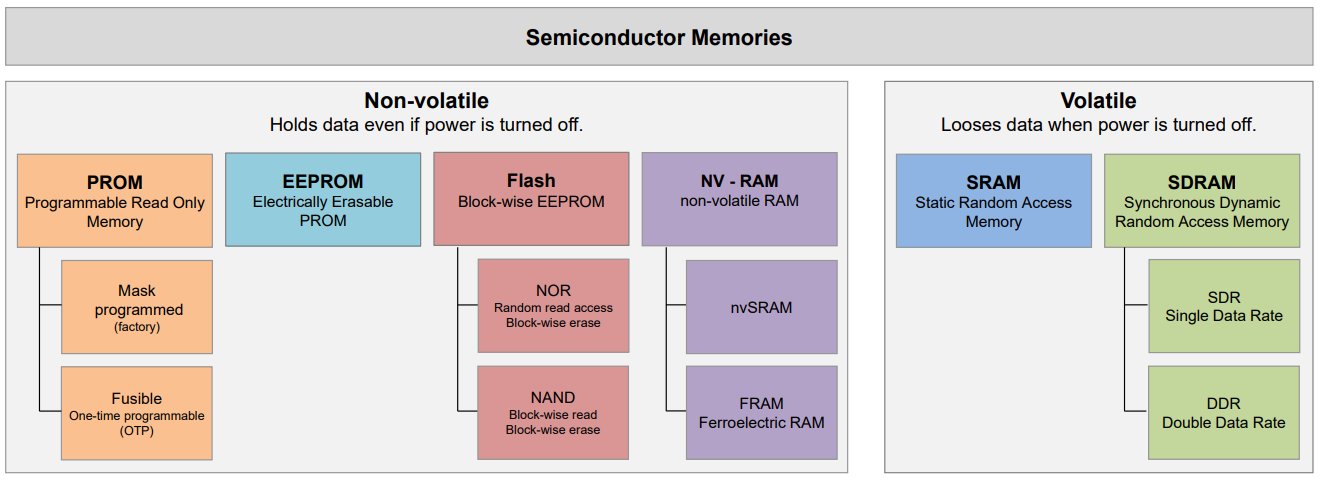
\includegraphics[width=\linewidth]{memorytechnologies.png}
\end{definition}

\mult{2}
\begin{concept}{Memory Organization} arrays of bit cells
\begin{itemize}
    \item \textbf{Array Size}: $n \times m$ (n words with m data bits)
    \item \textbf{Address Lines}: $k$ bits can address $2^k$ words
    \item \textbf{Data Lines}: Width of data bus (8, 16, 32 bits)
    \item \textbf{Control Lines}: Enable read/write operations
\end{itemize}
\end{concept}

\begin{corollary}{Hard Disk Storage Units} SI (metric) prefixes
    \begin{itemize}
        \item Kilo (k) = 1000 bytes
        \item Mega (M) = 1000 KiB = 1'000'000 bytes
        \item Giga (G) = 1000 MiB = 1'000'000'000 bytes
        \item Tera (T) = 1000 GiB = 1'000'000'000'000 bytes
    \end{itemize}
\end{corollary}

\begin{theorem}{Unit Symbols}
    \begin{itemize}
        \item b = bit
        \item B = Byte (8 bits)
    \end{itemize}
\end{theorem}

\begin{corollary}{Memory Chips and Prefixes}
    \begin{itemize}
        \item Kilo (K): KiB = 1024 bytes 
        \item Kib = Kibibyte = kilo binary byte
        \item Mega (M): MiB = 1024 KiB = 1'048'576 bytes
        \item Giga (G): GiB = 1024 MiB = 1'073'741'824 
        \item Tera (T): TiB = 1024 GiB = 1'099'511'627'776 
    \end{itemize}
\end{corollary}

\multend

\begin{concept}{Memory Architecture} nxm array (n words with m data bits each)

    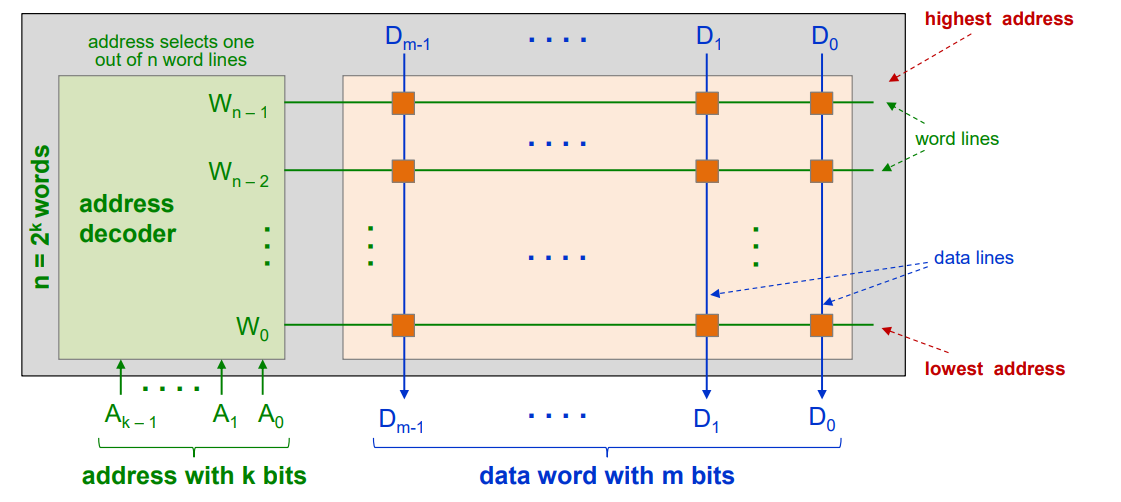
\includegraphics[width=\linewidth]{memoryarchitecturesize.png}

    \textcolor{tangerine}{Bit cell}: stores '0' or '1'

\end{concept}

\subsection{PROM, EEPROM, and Flash Memory}



\begin{concept}{PROM (Programmable Read-Only Memory)}
\begin{itemize}
    \item One-time programmable memory
    \item Programming involves physically altering the circuit (e.g., blowing fuses)
    \item Once programmed, contents cannot be changed
    \item Used for permanent storage of code or data
\end{itemize}
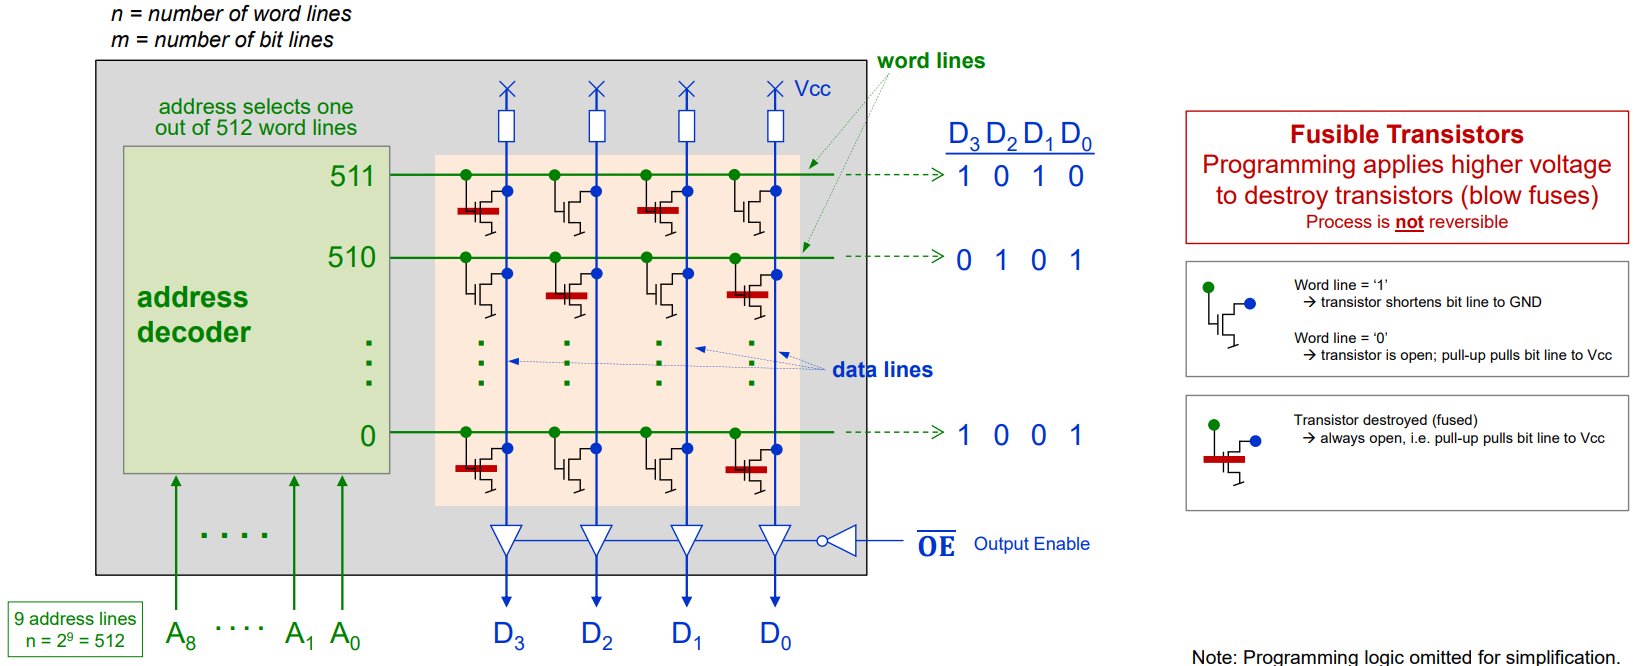
\includegraphics[width=\linewidth]{PROM.png}
\end{concept}

\begin{theorem}{Making PROMs Reprogrammable}\\
    'Floating Gate' transistor: Replace fusing by reprogrammable 'Floating Gate'
    \vspace{1mm}\\
Write cell to '0' $\rightarrow$ ON
\begin{itemize}
    \item High voltage (Up) deposits charge on the floating gate (isolated by SiO2)
    \item Transistor ON (conducting) if control gate equal '1'
\end{itemize}
\vspace{1mm}
Erase cell to '1' $\rightarrow$ OFF
\begin{itemize}
    \item Discharge floating gate (with negative Up)
    \item Transistor is OFF, i.e. blocking independent of value on the control gate
\end{itemize}
\end{theorem}

\begin{example2}{Use Floating Gates instead of Fusible Transistors}\\
    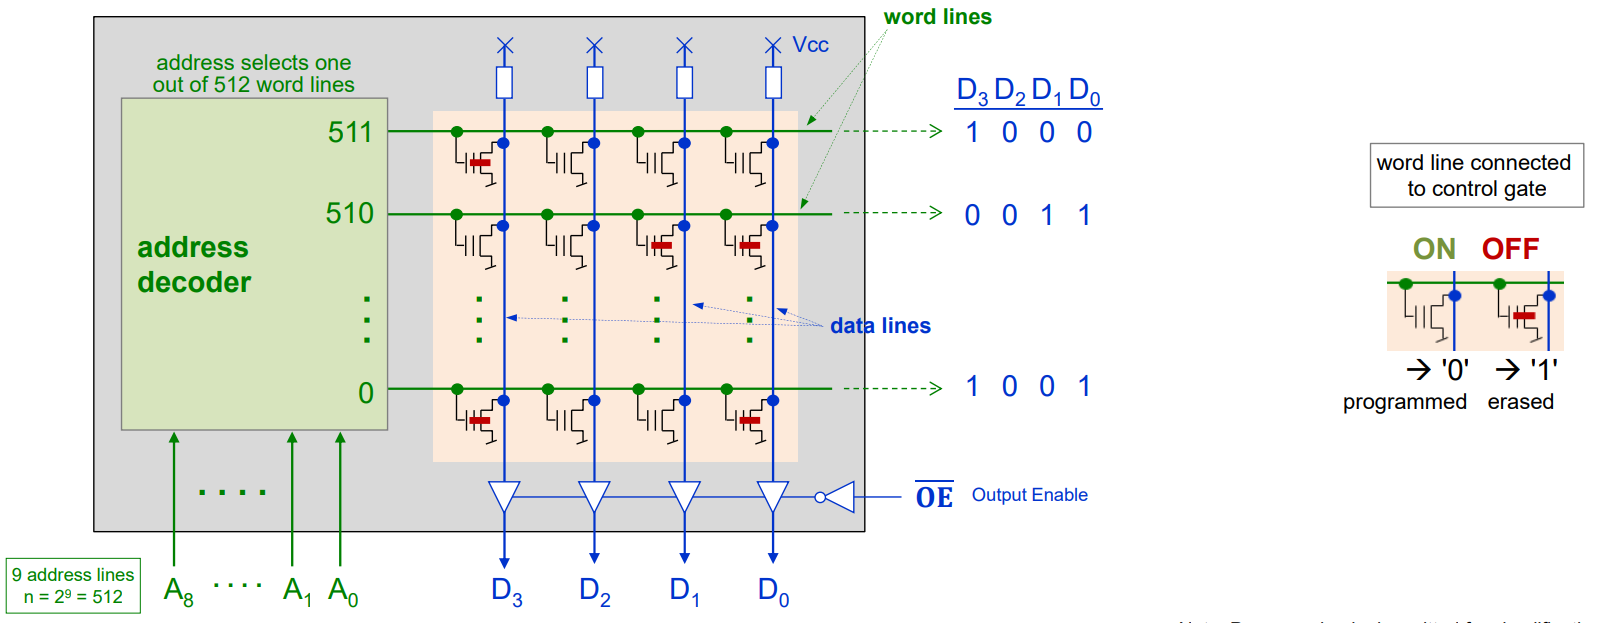
\includegraphics[width=\linewidth]{EEPROMandFlash.png}
\end{example2}


\begin{concept}{EEPROM (Electrically Erasable PROM)}\\
    High cell area $\rightarrow$ low density, high cost per bit
\begin{itemize}
    \item Uses floating-gate transistors to store data
    \item Can be electrically programmed and erased
    \item Byte-level erase and write operations
    \item Limited write cycles (typically 100,000 to 1,000,000)
    \item Slower and more expensive than SRAM
    \item Used for storing configuration data or parameters
\end{itemize}
\end{concept}

\begin{concept}{Flash Memory}\\
    Erasing can only be done for blocks, not individual bytes $\rightarrow$ small cell area, higher density than EEPROM, low cost per bit
\begin{itemize}
    \item Based on floating-gate transistor technology (like EEPROM)
    \item Higher density and lower cost per bit than EEPROM
    \item Block-wise erase operations (not byte-level)
    \item Write operations can only change bits from '1' to '0'
    \item Erase operations reset all bits in a block to '1'
    \item Limited write/erase cycles (typically 10,000 to 100,000)
    \item Used for code storage and mass data storage
\end{itemize}
\end{concept}


\begin{corollary}{Flash Memory Operations}\\
    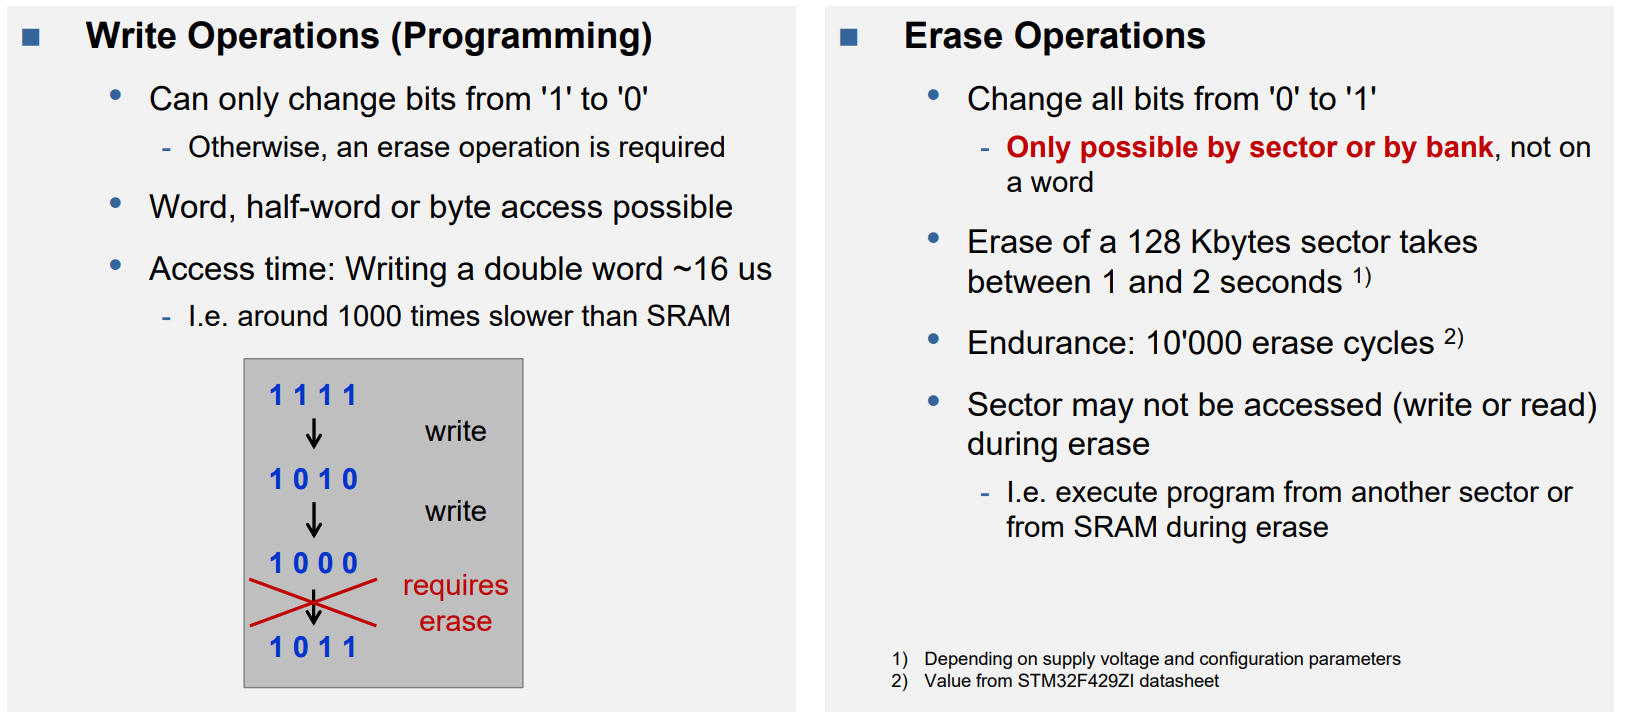
\includegraphics[width=\linewidth]{flashoperationsprom.png}
\end{corollary}



\begin{definition}{NOR vs. NAND Flash}

\begin{minipage}{0.5\linewidth}
\textbf{NOR Flash}:
\begin{itemize}
    \item Random access (like RAM)
    \item Execute-in-place capability (XIP)
    \item Fast read access
    \item Slow write and erase operations
    \item Lower density
    \item Used for code storage and execution
\end{itemize}
\end{minipage}
\begin{minipage}{0.5\linewidth}
\textbf{NAND Flash}:
\begin{itemize}
    \item Page-based access (not random)
    \item Cannot execute code directly
    \item Slow random read access
    \item Fast sequential read and write
    \item Higher density
    \item Used for mass storage (SSDs, memory cards)
\end{itemize}
\end{minipage}

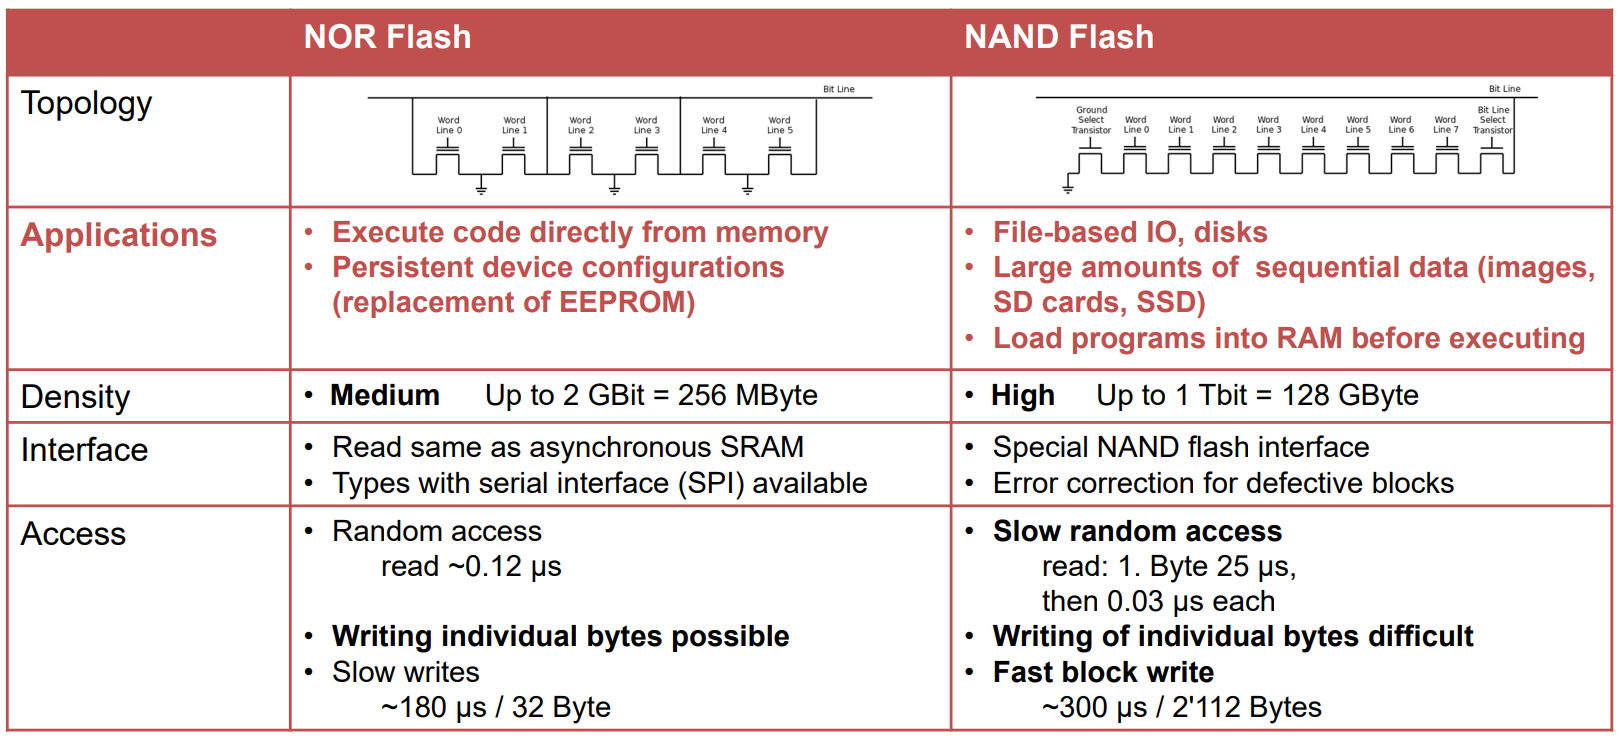
\includegraphics[width=\linewidth]{norvsnandflash.png}
\end{definition}

\begin{example2}{NOR vs. NAND Flash Applications}
    \textbf{NOR Flash - Anwendungen:}
    \begin{itemize}
        \item Mikrocontroller-Firmware (direkte Ausführung)
        \item BIOS/UEFI Code
        \item Embedded Systems mit wenig RAM
    \end{itemize}
    
    \textbf{NAND Flash - Anwendungen:}
    \begin{itemize}
        \item Solid State Drives (SSDs)
        \item SD-Karten, USB-Sticks
        \item Smartphones (App-Speicher)
    \end{itemize}
    
    \textbf{Wichtiger Unterschied:}
    NOR ermöglicht wahlfreie Zugriffe wie RAM, während NAND blockweise gelesen werden muss und eine spezielle Controller-Logik benötigt.
\end{example2}

\begin{remark}
    Bei der Speicher-Auswahl ist das Anwendungsprofil entscheidend: NOR Flash für direkten Code-Zugriff, NAND Flash für große Datenmengen, SRAM für schnelle Zwischenspeicherung, DRAM für große Arbeitsspeicher mit hoher Dichte.
\end{remark}

\raggedcolumns
\columnbreak

\subsection{SRAM (Static RAM)}

\mult{2}

\begin{concept}{SRAM Structure and Characteristics}
\begin{itemize}
    \item Uses flip-flop circuit for each bit \\ (typically 6 transistors)
    \item Maintains data as long as power is supplied
    \item No refresh required (unlike DRAM)
    \item Fast access times (a few nanoseconds)
    \item Low power consumption in standby mode
    \item Higher cost and lower density than DRAM
    \item Used for cache memory and high-speed buffers
\end{itemize}
\end{concept}

\begin{definition}{SRAM Cell}
\begin{itemize}
    \item Cross-coupled inverters forming a latch to store one bit
    \item 2 access transistors to connect cell to bit lines
    \item Word line to enable/disable access to the cell
    \item High state ('1') and low state ('0') stable as long as power is maintained
\end{itemize}
\end{definition}

\multend

\begin{theorem}{SRAM Operations}

\begin{minipage}{0.5\linewidth}
\textbf{Read Operation}:
\begin{itemize}
    \item Word line is activated
    \item Access transistors connect cell to bit lines
    \item Sense amplifiers detect voltage difference on bit lines
    \item Data is read from bit lines
\end{itemize}
\end{minipage}
\begin{minipage}{0.5\linewidth}
\textbf{Write Operation}:
\begin{itemize}
    \item Word line is activated
    \item Access transistors connect cell to bit lines
    \item Write drivers force bit lines to desired values
    \item Cell state changes to match bit line values
\end{itemize}
\end{minipage}
\end{theorem}





\begin{corollary}{SRAM Write Operation}\\
    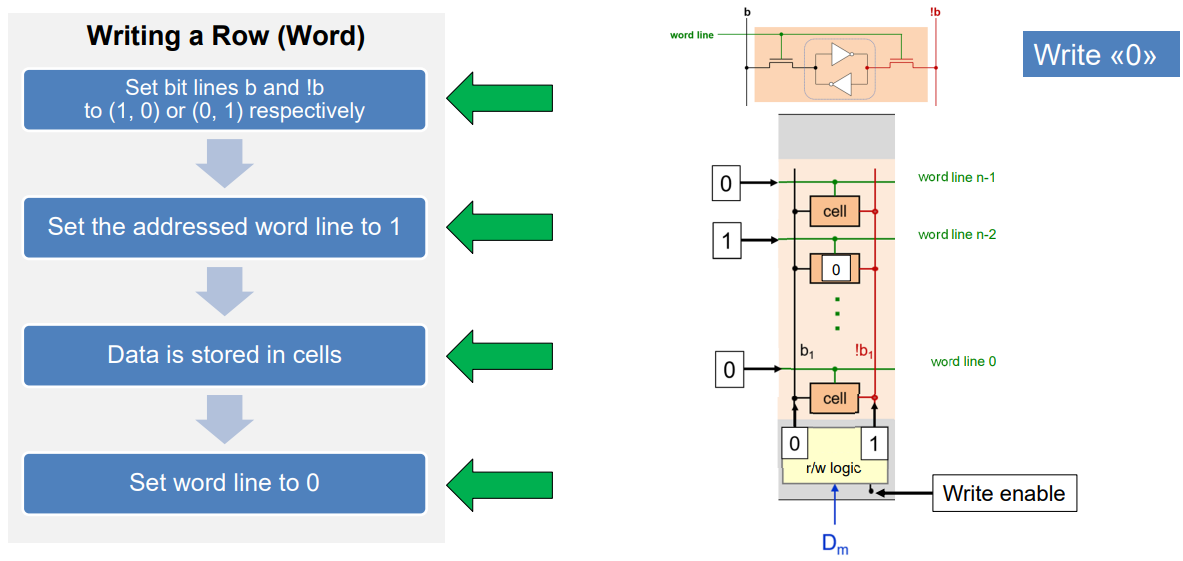
\includegraphics[width=0.7\linewidth]{sramwrite.png}
\end{corollary}

\begin{corollary}{SRAM Read Operation}\\
    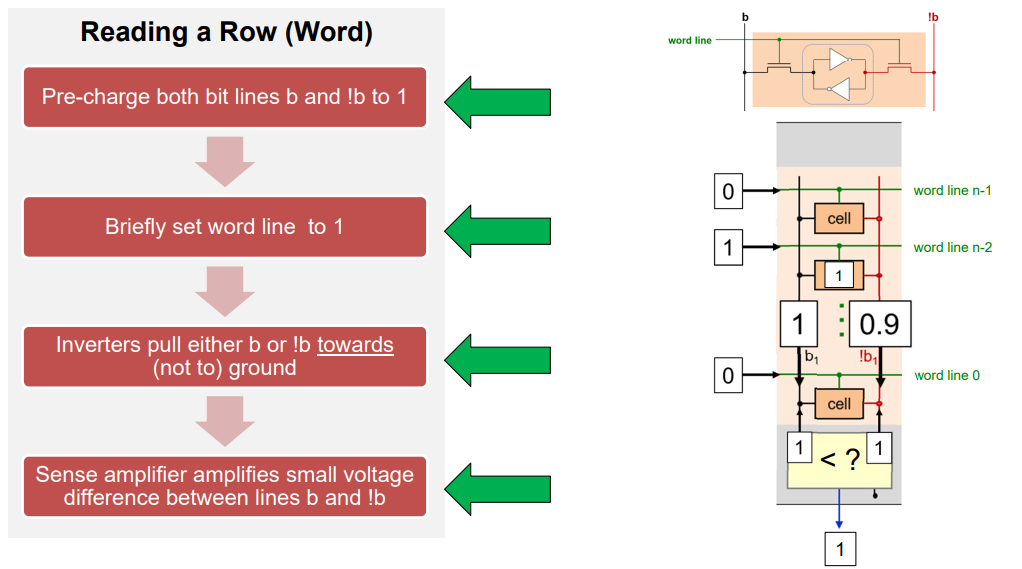
\includegraphics[width=0.7\linewidth]{sramread.png}
\end{corollary}

\begin{definition}{Asynchronous SRAM Interface}\\
Asynchronous SRAM devices typically have these control signals:
\begin{itemize}
    \item \textbf{CS} (Chip Select): Enables the memory device (active low)
    \item \textbf{OE} (Output Enable): Enables data output during read (active low)
    \item \textbf{WE} (Write Enable): Indicates write operation (active low)
    \item \textbf{Address Lines}: Select memory location
    \item \textbf{Data Lines}: Bidirectional lines for data transfer
\end{itemize}
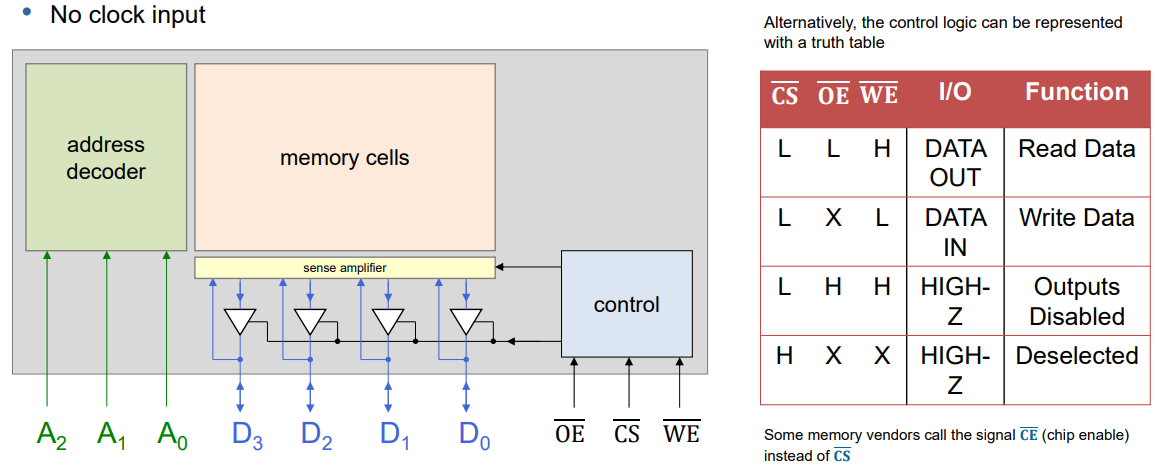
\includegraphics[width=\linewidth]{asyncsram.png}\\
Read: $\overline{\mathrm{CS}}=0 \mathrm{AND} \overline{\mathrm{OE}}=0 \mathrm{AND} \overline{\mathrm{WE}}=1$\\
Write: $\overline{\mathrm{CS}}=0 \mathrm{AND} \overline{\mathrm{WE}}=0$
\end{definition}

\subsection{SDRAM (Synchronous DRAM)}



\begin{concept}{SDRAM Structure and Characteristics}
\begin{itemize}
    \item Uses a capacitor and one transistor for each bit
    \item Requires periodic refresh to maintain data (capacitor leakage)
    \item Synchronous interface (clocked)
    \item Row and column addressing (multiplexed address bus)
    \item Higher density and lower cost than SRAM
    \item Higher power consumption due to refresh
    \item Used for main memory in computers and embedded systems
\end{itemize}

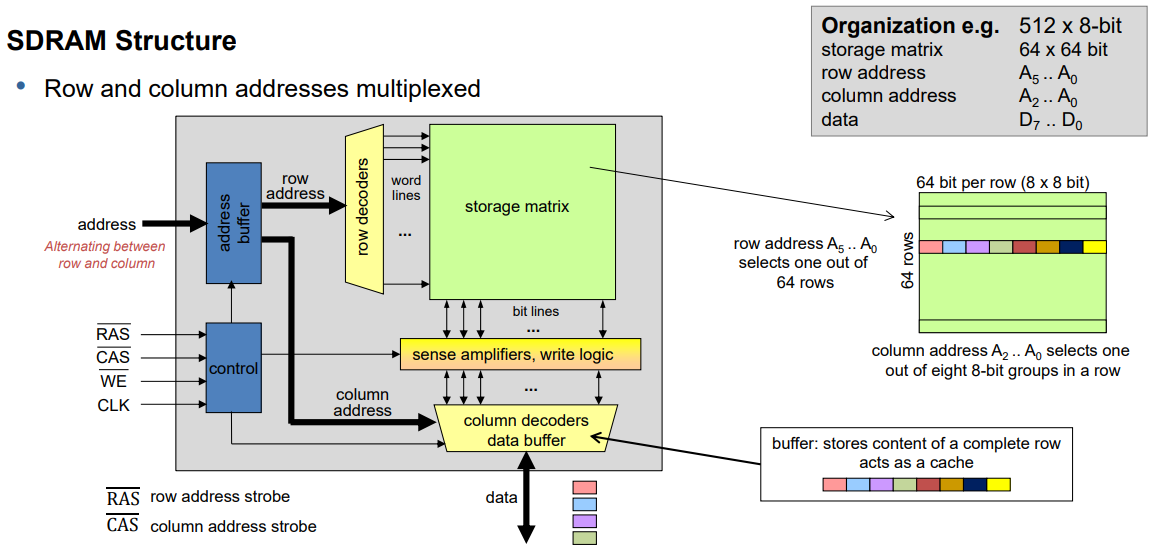
\includegraphics[width=\linewidth]{sdramstructure.png}
\end{concept}

\begin{definition}{SDRAM Operation}\\
Key aspects of SDRAM operation:
\begin{itemize}
    \item \textbf{Refresh}: Periodic read and rewrite of all memory cells
    \item \textbf{Row Activation}: Opening a row copies data to row buffer
    \item \textbf{Column Access}: Selecting specific bytes from row buffer
    \item \textbf{Precharge}: Preparing a bank for next row activation
    \item \textbf{Burst Mode}: Sequential access to multiple columns
\end{itemize}
\end{definition}


\begin{theorem}{SDRAM Timing} Multiplexed row and column addresses, clocks up to 1200 MHz\\
    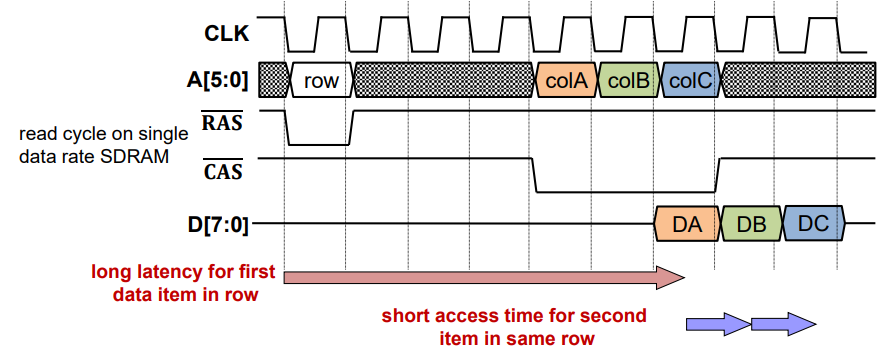
\includegraphics[width=0.8\linewidth]{sdramtiming.png}\\
    RAS low: Master places the 6-bit row address on lines A[5:0]\\
    CAS low: Master places the 3-bit column address on lines A[2:0], lines A[5:3] are unused
\end{theorem}

\begin{corollary}{SRAM vs. SDRAM Comparison}
\begin{center}
\begin{tabular}{|p{3cm}|p{4cm}|p{4cm}|}
\hline
\textbf{Feature} & \textbf{SRAM} & \textbf{SDRAM} \\
\hline
Cell Structure & 6 transistors (flip-flop) & 1 transistor + 1 capacitor \\
\hline
Refresh & Not required & Required (periodic) \\
\hline
Density & Lower & Higher \\
\hline
Cost per bit & Higher & Lower \\
\hline
Access Time & Faster, uniform & Variable (row hit vs. miss) \\
\hline
Interface & Often asynchronous & Synchronous (clocked) \\
\hline
Power Consumption & Lower static power & Higher due to refresh \\
\hline
Applications & Cache, high-speed buffer & Main memory \\
\hline
\end{tabular}
\end{center}

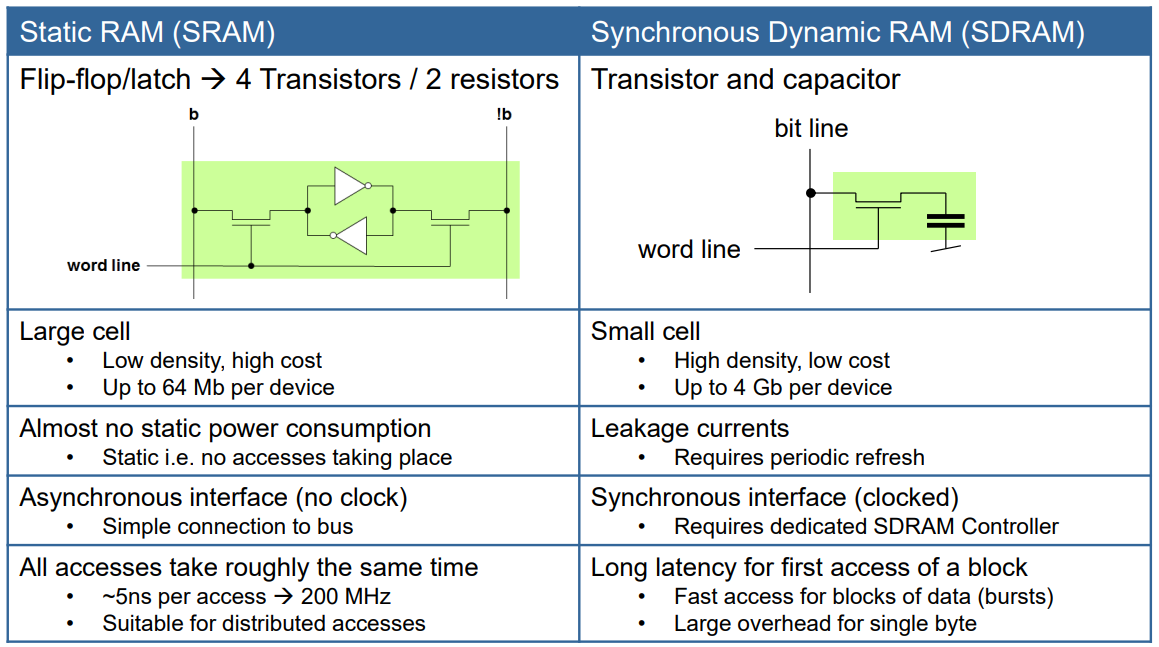
\includegraphics[width=0.8\linewidth]{sramvssdram.png}
\end{corollary}


\subsection{Memory Technology Comparison}



\begin{concept}{SRAM vs. SDRAM Unterschiede}
    \paragraph{Speichertyp}
    \begin{itemize}
        \item SRAM: Statisch (Flip-Flop basiert)
        \item SDRAM: Dynamisch (Kondensator basiert)
    \end{itemize}
    
    \paragraph{Refresh-Verhalten}
    \begin{itemize}
        \item SRAM: Stores data as long as power is applied, without requiring refresh.
        \item SDRAM: Stores data as charge in a capacitor that leaks over time. Requires periodic refresh to maintain data integrity.
    \end{itemize}
    
    \paragraph{Schnittstelle}
    \begin{itemize}
        \item SRAM: Asynchron (NWE, NOE Signale)
        \item SDRAM: Synchron (RAS, CAS Signale, getaktet)
    \end{itemize}
    
    \paragraph{Zugriffszeit und Timing}
    \begin{itemize}
        \item SRAM: Provides fast random access with consistent timing for all accesses (~5ns). All operations take roughly the same time.
        \item SDRAM: Synchronous interface with clock. Has higher latency for first access in a row (~60ns), but very fast subsequent access within same row. Optimized for burst transfers.
    \end{itemize}
    
    \paragraph{Speicherdichte und Kosten}
    \begin{itemize}
        \item SRAM: Low density due to large cell size (6 transistors). Higher cost per bit. Typically limited to 64Mb per device.
        \item SDRAM: High density due to small cell size (1 transistor + 1 capacitor). Lower cost per bit. Can reach 4Gb or more per device.
    \end{itemize}

\paragraph{Typical applications:}
   \begin{itemize}
     \item SRAM: CPU cache memory, small buffer memory, applications requiring fast random access.
     \item SDRAM: Main system memory, large buffers, applications requiring high capacity with reasonable access speed.
   \end{itemize}

    \textbf{OE-Pin Funktion bei SRAM:}
    Kontrolliert, ob das Memory Daten auf den Bus treibt oder ob sich die Ausgangstreiber im Floating-Zustand befinden.
\end{concept}

\begin{example2}{DRAM-Eigenschaften bewerten}
    \paragraph{Speicherzelle}
    \begin{itemize}
        \item \textcolor{frog}{$\checkmark$} Kondensator + Transistor (nicht RS Flip-Flop)
        \item \textcolor{frog}{$\checkmark$} Sehr kleine Zelle $\rightarrow$ hohe Dichte
    \end{itemize}
    
    \paragraph{Zugriffsmuster}
    \begin{itemize}
        \item \textcolor{frog}{$\checkmark$} Hohe Latenz für einzelne Zugriffe
        \item \textcolor{frog}{$\checkmark$} Optimiert für Blockzugriffe (Burst)
    \end{itemize}
    
    \paragraph{Refresh und Leistung}
    \begin{itemize}
        \item \textcolor{frog}{$\checkmark$} Periodischer Refresh wegen Leckströmen
        \item \textcolor{frog}{$\checkmark$} Volatiler Speicher
        \item \textcolor{red}{$\times$} Kein niedriger Leistungsverbrauch (Refresh erforderlich)
    \end{itemize}
    
    \paragraph{Kosten}
    \begin{itemize}
        \item \textcolor{red}{$\times$} Niedriger Preis pro Speicherzelle (nicht hoch)
    \end{itemize}
\end{example2}

\begin{KR}{Comparing Memory Technologies}
\paragraph{Identify memory characteristics}
\begin{itemize}
    \item \textbf{Volatility:} Whether memory loses contents when power is removed
    \begin{itemize}
        \item \textit{Volatile:} SRAM, DRAM/SDRAM
        \item \textit{Non-volatile:} PROM, EEPROM, Flash, NV-RAM
    \end{itemize}
    \item \textbf{Storage mechanism:} How bits are physically stored
    \begin{itemize}
        \item \textit{SRAM:} Flip-flop-based cells (6 transistors)
        \item \textit{DRAM:} Capacitor-based cells (1 transistor + 1 capacitor)
        \item \textit{Flash:} Floating-gate transistors
    \end{itemize}
    \item \textbf{Access method:} How data is accessed
    \begin{itemize}
        \item \textit{Random access:} Any location accessed in the same time (SRAM, NOR Flash)
        \item \textit{Block access:} Efficient for large blocks (NAND Flash)
        \item \textit{Sequential access:} Fast for sequential data (SDRAM with burst mode)
    \end{itemize}
\end{itemize}

\paragraph{Compare memory performance metrics}
\begin{itemize}
    \item \textbf{Access time:} Time to read/write data
    \begin{itemize}
        \item SRAM: 2-10ns
        \item SDRAM: 60ns+ for first access, then fast for burst
        \item NOR Flash: \~120ns read
        \item NAND Flash: Slow random access (25$\mu$s first byte)
    \end{itemize}
    \item \textbf{Density:} Storage capacity per unit area
    \begin{itemize}
        \item SRAM: Low (large cells, expensive)
        \item DRAM: High (small cells, inexpensive)
        \item NAND Flash: Very high (highest density, lowest cost per bit)
    \end{itemize}
    \item \textbf{Power consumption:} Energy required for operation
    \begin{itemize}
        \item SRAM: Low static power (no refresh needed)
        \item DRAM: Higher (requires refresh)
        \item Flash: Very low when not being written/erased
    \end{itemize}
\end{itemize}

\paragraph{Analyze application suitability}
\begin{itemize}
    \item \textbf{SRAM:} Cache memory, small temporary storage
    \item \textbf{DRAM/SDRAM:} Main memory, large temporary storage
    \item \textbf{NOR Flash:} Program code storage, direct execution
    \item \textbf{NAND Flash:} Mass storage, data logging, SSD drives
\end{itemize}
\end{KR}

\begin{concept}{NOR vs. NAND Flash Vergleich}
    \paragraph{NOR Flash}
    \begin{itemize}
        \item \textcolor{frog}{$\checkmark$} Direkter Code-Execution (XIP - Execute in Place)
        \item \textcolor{frog}{$\checkmark$} Wahlfreie Byte-Zugriffe
        \item \textcolor{frog}{$\checkmark$} SRAM-kompatible Schnittstelle
        \item \textcolor{frog}{$\checkmark$} Bits einzeln auf '0' schreibbar
        \item \textcolor{frog}{$\checkmark$} Für Programmcode und persistente Daten
        \item \textcolor{red}{$\times$} Nicht für große Datenblöcke optimiert
    \end{itemize}
    
    \paragraph{NAND Flash}
    \begin{itemize}
        \item \textcolor{frog}{$\checkmark$} Effizient für große Datenblöcke
        \item \textcolor{frog}{$\checkmark$} Hohe Schreibgeschwindigkeit für Blöcke
        \item \textcolor{frog}{$\checkmark$} Spezielle Schnittstelle (nicht SRAM-kompatibel)
        \item \textcolor{frog}{$\checkmark$} Hohe Latenz für ersten Zugriff
        \item \textcolor{frog}{$\checkmark$} Für SSDs verwendet
        \item \textcolor{red}{$\times$} Code muss ins RAM geladen werden
        \item \textcolor{red}{$\times$} Keine wahlfreien Byte-Zugriffe
    \end{itemize}
    
    \paragraph{Gemeinsame Eigenschaften}
    \begin{itemize}
        \item \textcolor{frog}{$\checkmark$} Floating Gate Technologie
        \item \textcolor{frog}{$\checkmark$} Nur sektorweises Löschen auf '1'
        \item \textcolor{red}{$\times$} Bits können nicht einzeln auf '1' geschrieben werden
    \end{itemize}
\end{concept}


\raggedcolumns
\columnbreak

\subsection{STM32F4 On-Chip Memory}

\begin{concept}{STM32F4 Memory Architecture}\\
The STM32F429ZI microcontroller includes:

\begin{minipage}{0.65\linewidth}
\textbf{Flash Memory}: 2 MB (program storage)
    \begin{itemize}
        \item NOR topology with execute-in-place capability
        \item Divided into sectors of varying sizes (16KB to 128KB)
        \item Organized in two banks for read-while-write operations
        \item Non-volatile storage (retains data without power)
        \item Store code and persistent data
    \end{itemize}
\end{minipage}
\begin{minipage}{0.35\linewidth}
\textbf{SRAM}: 256 KB total
    \begin{itemize}
        \item SRAM1: 112 KB
        \item SRAM2: 16 KB
        \item SRAM3: 64 KB
        \item CCM (Core Coupled Memory): \\ 64 KB (accessible only by CPU)
        \\ $\rightarrow$ Fast access, low latency
    \end{itemize}
\end{minipage}
\end{concept}

\begin{definition}{STM32F4 Flash Characteristics}
\begin{itemize}
    \item \textbf{Write Operations}: Can only change bits from '1' to '0'
    \item \textbf{Erase Operations}: Resets all bits in a sector to '1'
    \item \textbf{Programming Time}: Around 16µs per double word
    \item \textbf{Erase Time}: 1-2 seconds for a 128KB sector
    \item \textbf{Endurance}: 10,000 erase cycles
    \item \textbf{Access Time}: Higher latency than SRAM (requires up to 8 wait states on on-chip bus)
    \item \textbf{Pre-Fetch Queue}: ST uses 128-bit buffer with pre-fetch queue, reduces performance penalty when executing sequential instructions
\end{itemize}
\end{definition}

\mult{2}

\begin{theorem}{SRAM on-chip memory}\\
    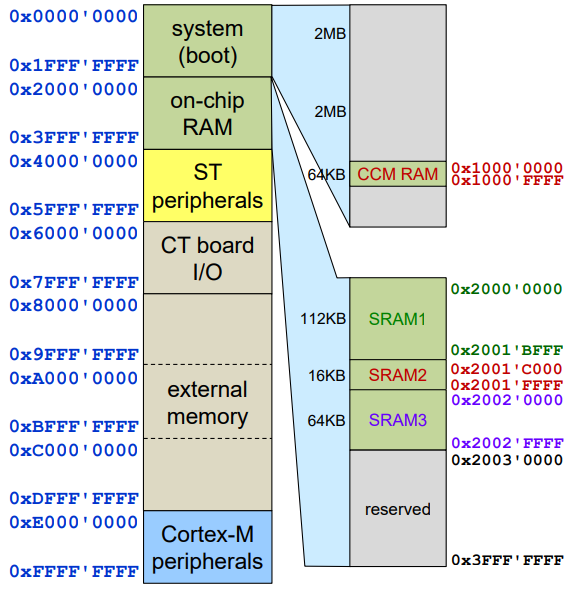
\includegraphics[width=0.9\linewidth]{sramonchip.png}
\end{theorem}

\begin{theorem}{Flash on-chip memory}\\
    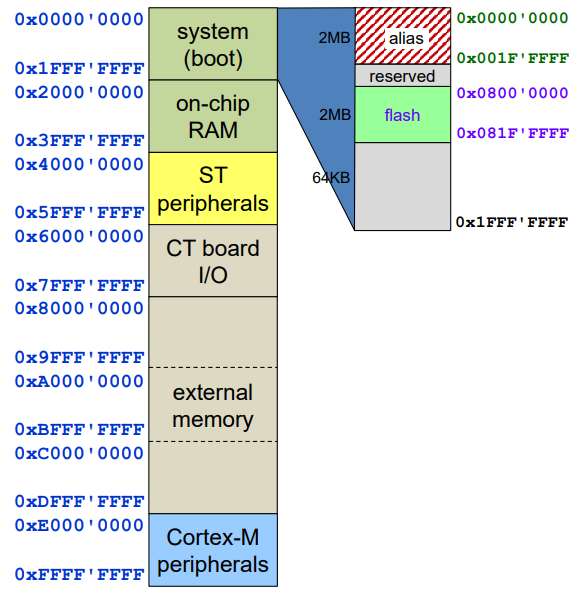
\includegraphics[width=0.9\linewidth]{flashonchip.png}
\end{theorem}

\multend

\begin{corollary}{Flash is partitioned into sectors}
    \begin{itemize}
        \item Sectors can only be erased as a whole
        \item Writing through control registers - no direct memory write access
    \end{itemize}
    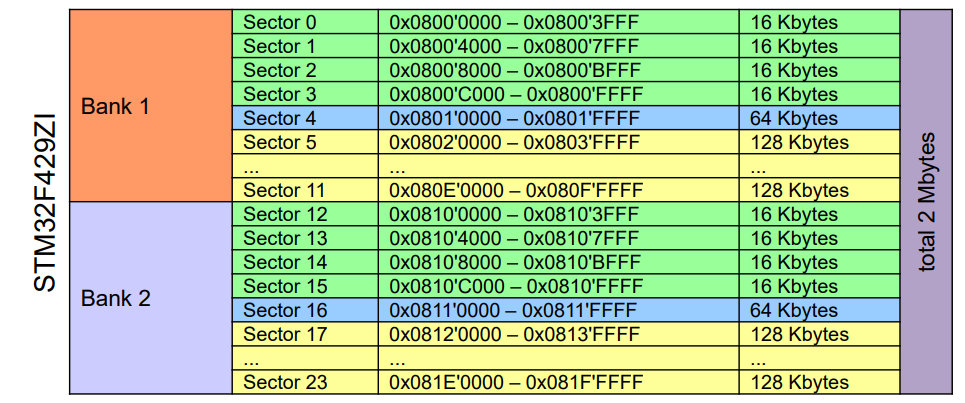
\includegraphics[width=0.8\linewidth]{flashsecrotrs.png}
\end{corollary}



\subsection{External Memory (off-chip)}

\mult{2}

\begin{concept}{Flexible Memory Controller (FMC)}
\begin{itemize}
    \item Interface between on-chip system bus and \\ external memory devices
    \item Support for different memory types:
    \begin{itemize}
        \item SRAM, NOR Flash, PSRAM
        \item NAND Flash
        \item SDRAM
    \end{itemize}
    \item Configurable bus width (8, 16, or 32 bits)
    \item Programmable timing parameters
    \item Memory banking with up to 6 banks
\end{itemize}
\end{concept}

\begin{definition}{FMC Signals}\\
Key FMC signals for external SRAM/NOR flash:
\begin{itemize}
    \item \textbf{A[25:0]}: Address bus $\rightarrow$ OUT
    \item \textbf{D[31:0]}: Data bus (bidirectional) $\rightarrow$ OUT/IN
    \item \textbf{NE[4:1]}: Chip enable signals (active low) \\ $\rightarrow$ OUT
    \item \textbf{NOE}: Output enable (active low) $\rightarrow$ OUT
    \item \textbf{NWE}: Write enable (active low) $\rightarrow$ OUT
    \item \textbf{NBL[3:0]}: Byte lane enables (active low)
\end{itemize}

\end{definition}

\multend

\begin{example2}{Connecting an external 8-bit asynchronous SRAM device}\\
    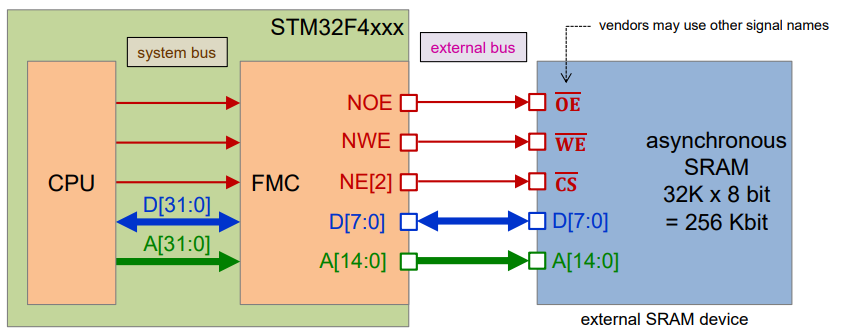
\includegraphics[width=0.7\linewidth]{scmsramexmaple.png}
\end{example2}

\begin{concept}{External Memory Access}
    Different number data lines cause bottle necks

\begin{minipage}{0.4\linewidth}
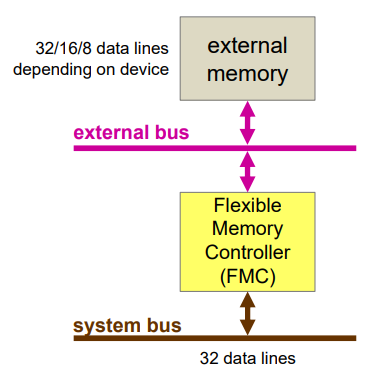
\includegraphics[width=0.8\linewidth]{fmc.png}
\end{minipage}
\begin{minipage}{0.6\linewidth}
\textbf{Write Operations}:
\begin{itemize}
    \item CPU write stored in FMC FIFO buffer
    \item System bus released for other access
    \item FMC completes external write(s)
\end{itemize}
\textbf{Read Operations}:
\begin{itemize}
    \item System bus must wait until all external reads complete
    \item Multiple external cycles for narrow memory widths
\end{itemize}
Accessing external memory with different bus widths:
\begin{itemize}
    \item \textbf{32-bit CPU Access to 32-bit Memory}: 1 external bus cycle
    \item \textbf{32-bit CPU Access to 16-bit Memory}: 2 external bus cycles
    \item \textbf{32-bit CPU Access to 8-bit Memory}: 4 external bus cycles
\end{itemize}
\end{minipage}
\end{concept}

\begin{example2}{FMC Write Operation}\\
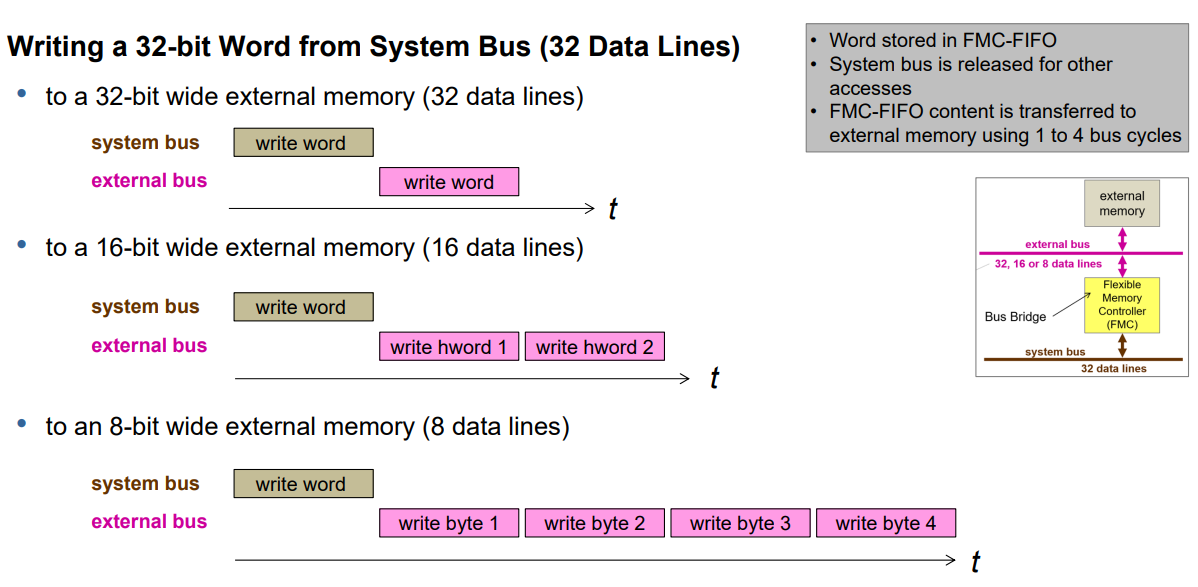
\includegraphics[width=0.9\linewidth]{fmcexample1.png}
\end{example2}

\begin{example2}{FMC Read Operation}\\
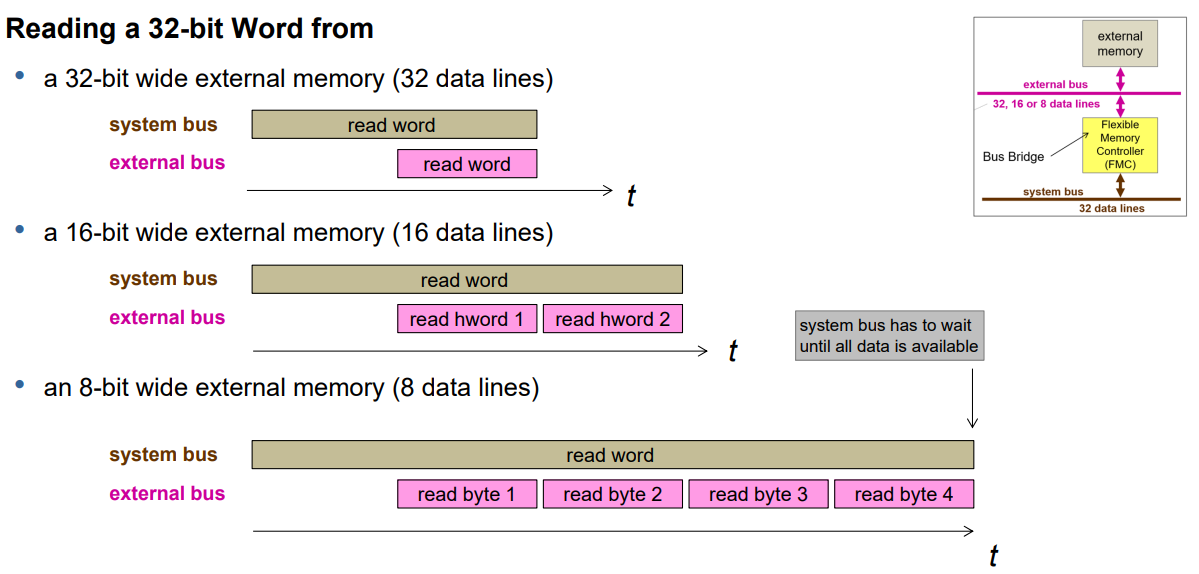
\includegraphics[width=0.9\linewidth]{fmcexample2.png}
\end{example2}

\subsubsection{External Memory Configuration}

\begin{concept}{Memory Banks}\\
    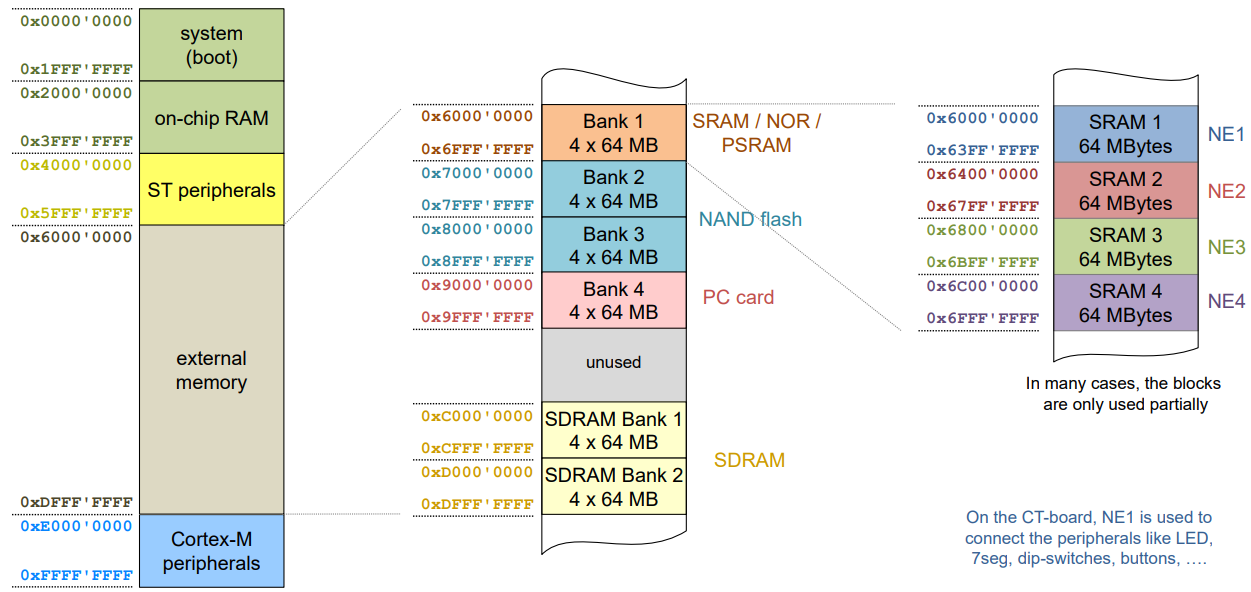
\includegraphics[width=\linewidth]{memorybanks.png}\\
    \important{Alternative view in SEP Handout (FMC Decoding)}
\end{concept}

\begin{KR}{Connecting External Memory to STM32}
\paragraph{Identify external memory type and requirements}
\begin{itemize}
    \item Determine memory interface type (asynchronous SRAM, NOR Flash, NAND Flash, SDRAM)
    \item Identify memory capacity and organization (width x depth)
    \item Note timing requirements from datasheet
\end{itemize}

\paragraph{Configure FMC (Flexible Memory Controller)}
\begin{itemize}
    \item Enable FMC clock in RCC registers
    \item Configure memory bank registers based on memory type:
    \begin{itemize}
        \item Bank 1-4: SRAM/NOR/PSRAM (BCRx and BTRx registers)
        \item Bank 5-6: SDRAM (SDCR and SDTR registers)
    \end{itemize}
    \item Set data bus width (8/16/32 bits)
    \item Configure timing parameters:
    \begin{itemize}
        \item ADDSET: Address setup time
        \item DATAST: Data setup time
        \item BUSTURN: Bus turnaround time
    \end{itemize}
\end{itemize}

\paragraph{Configure GPIO pins for FMC}
\begin{itemize}
    \item Enable GPIO clocks in RCC registers
    \item Configure GPIO pins for alternate function (FMC)
    \item Set GPIO speed, typically high or very high
\end{itemize}

\paragraph{Understand memory mapping}
\begin{itemize}
    \item Know the address ranges for each FMC bank:
    \begin{itemize}
        \item Bank 1: 0x6000 0000 - 0x6FFF FFFF
        \item Bank 2: 0x7000 0000 - 0x7FFF FFFF
        \item Bank 3: 0x8000 0000 - 0x8FFF FFFF
        \item Bank 4: 0x9000 0000 - 0x9FFF FFFF
        \item SDRAM Bank 1: 0xC000 0000 - 0xCFFF FFFF
        \item SDRAM Bank 2: 0xD000 0000 - 0xDFFF FFFF
    \end{itemize}
    \item Understand chip select logic (NE1-NE4)
    \item Account for memory width in address calculations
\end{itemize}
\end{KR}



\subsubsection{Connecting Asynchronous SRAM to STM32F4}

\begin{concept}{Connecting Asynchronous SRAM to STM32F4}
\paragraph{Step 1: Configure GPIO pins}
Set the GPIO pins for FMC signals to alternate function mode.
\paragraph{Step 2: Configure FMC timing}
Set appropriate timing parameters (ADDSET, DATAST) based on memory datasheet.
\paragraph{Step 3: Configure FMC bank}
Set the memory type, data width, and other parameters.
\paragraph{Step 4: Enable FMC}
Enable the FMC peripheral.

\begin{lstlisting}[language=C, style=basesmol]
// Configure external SRAM (16-bit) on FMC bank 1

// Step 1: Configure GPIO pins for FMC
// Enable GPIO clocks
RCC->AHB1ENR |= RCC_AHB1ENR_GPIODEN | RCC_AHB1ENR_GPIOEEN |
                RCC_AHB1ENR_GPIOFEN | RCC_AHB1ENR_GPIOGEN;

// Configure GPIO pins (example for some pins)
// Set alternate function mode (0x2)
GPIOD->MODER |= 0x55555555;  // All pins to alternate function
GPIOE->MODER |= 0x55555555;
// Set to AF12 (FMC)
GPIOD->AFR[0] = 0xCCCCCCCC;
GPIOD->AFR[1] = 0xCCCCCCCC;
GPIOE->AFR[0] = 0xCCCCCCCC;
GPIOE->AFR[1] = 0xCCCCCCCC;

// Step 2: Enable FMC clock
RCC->AHB3ENR |= RCC_AHB3ENR_FMCEN;

// Step 3: Configure FMC bank 1 for SRAM
// Set timing for SRAM (example values)
FMC_Bank1->BTCR[0] = 
    FMC_BCR1_MBKEN |    // Memory bank enable
    FMC_BCR1_MTYP_0 |   // Memory type SRAM
    FMC_BCR1_MWID_0 |   // 16-bit data bus
    FMC_BCR1_WREN;      // Write enable

// Set timing (ADDSET=1, DATAST=2)
FMC_Bank1->BTCR[1] = 
    (1 << FMC_BTR1_ADDSET_Pos) |
    (2 << FMC_BTR1_DATAST_Pos);
\end{lstlisting}
\end{concept}



\begin{example2}{Connecting Asynchronous SRAM to STM32F4}\\
    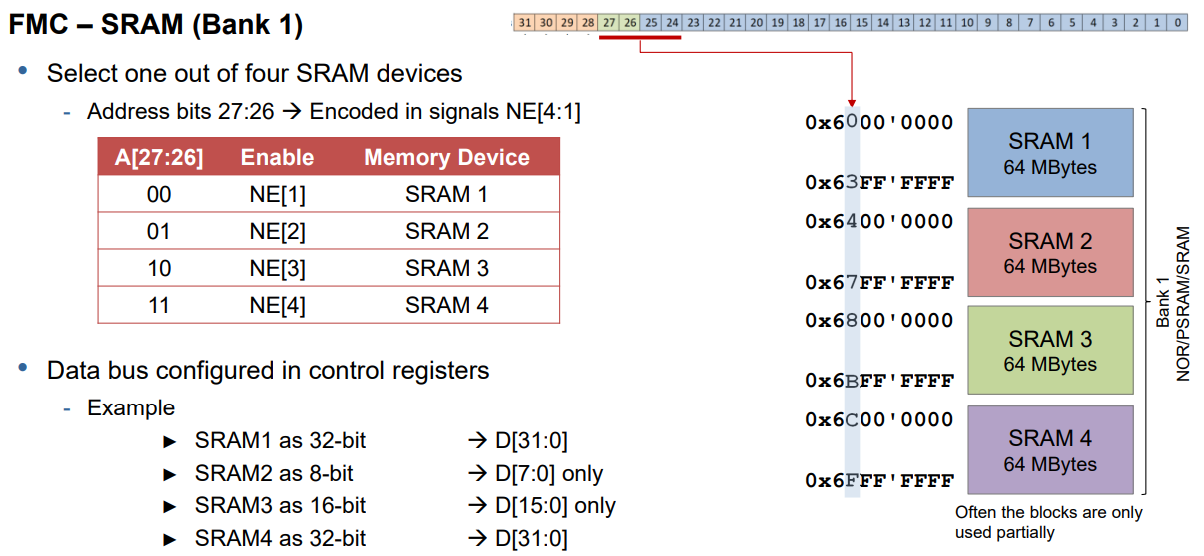
\includegraphics[width=\linewidth]{fmcsramex1.png}
\end{example2}

\begin{example2}{Timing on external bus} as seen from the microcontroller\\
    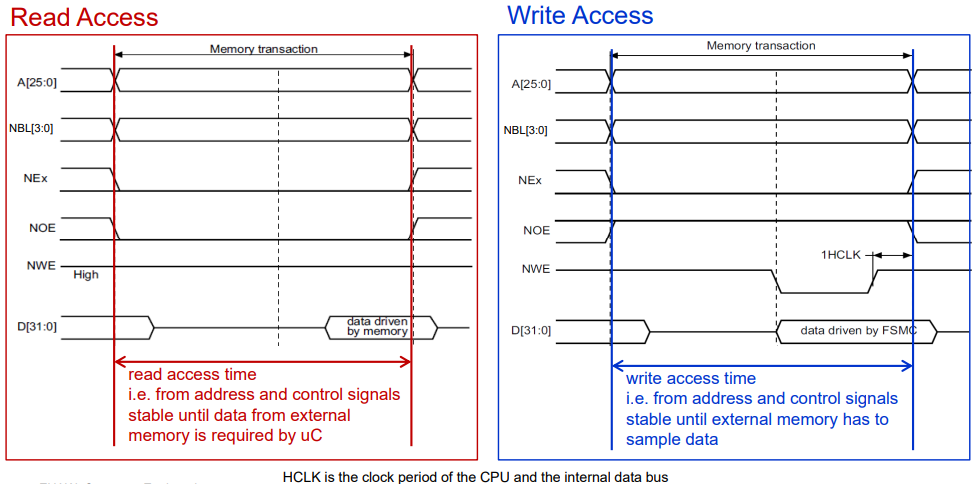
\includegraphics[width=\linewidth]{timingsramex.png}
\end{example2}

\begin{example2}{FMC Configuration for Asynchronous SRAM}\\
    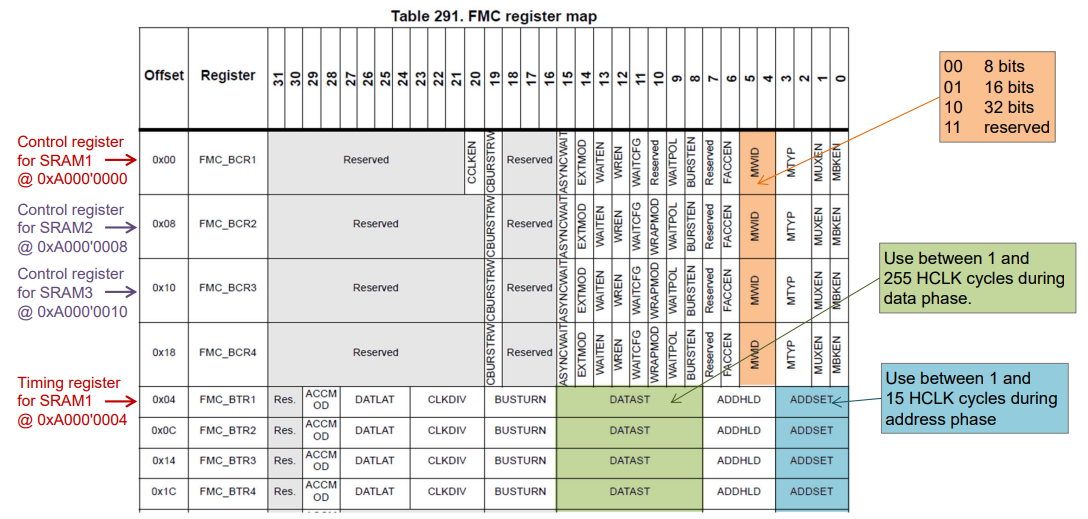
\includegraphics[width=\linewidth]{fmcsrawmex.png}
\end{example2}

\begin{concept}{Different Data Bus Widths}\\
    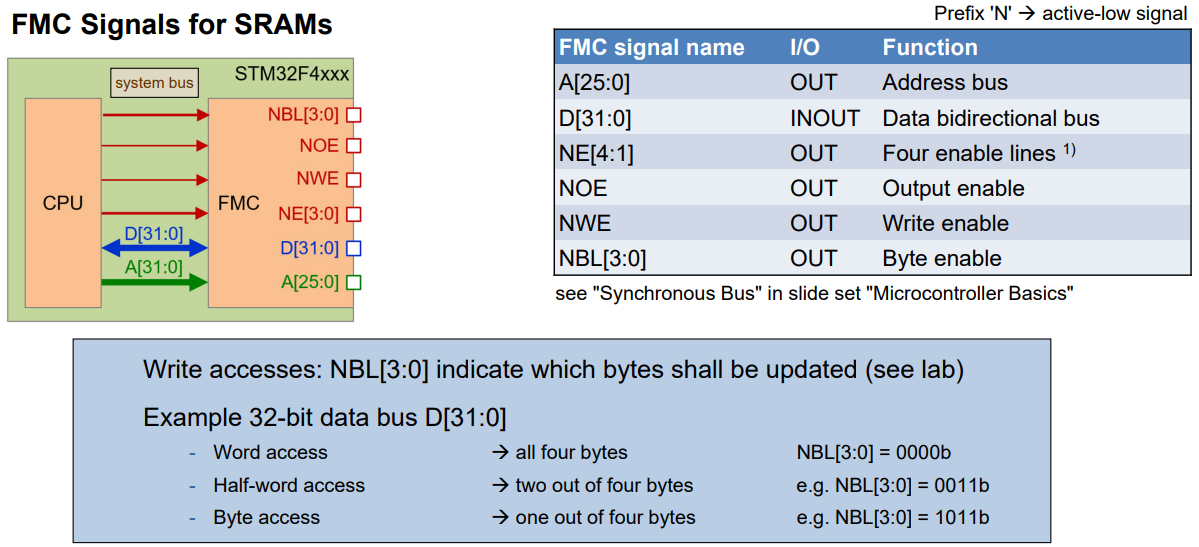
\includegraphics[width=\linewidth]{buswidthssram.png}
\end{concept}




\subsection{Memory Access and Address Decomposition}

\begin{KR}{Analyzing Memory Access Patterns}
\paragraph{Determine memory access type}
\begin{itemize}
    \item Identify memory type and organization (width × depth)
    \item Determine CPU data bus width (typically 32-bit for Cortex-M)
    \item Identify the size of the access (byte, half-word, word)
\end{itemize}

\paragraph{Memory address decomposition}
\begin{itemize}
    \item Identify bank select bits from address (typically bits 27:26)
    \begin{itemize}
        \item 00: Bank 1, 01: Bank 2, 10: Bank 3, 11: Bank 4
    \end{itemize}
    \item Identify chip enable from bank and address
    \begin{itemize}
        \item Within each bank, specific regions activate NE1-NE4
    \end{itemize}
    \item Determine memory location within the device (lower address bits)
\end{itemize}

\paragraph{Analyze byte enables for sub-word accesses}
\begin{itemize}
    \item For 32-bit data bus: NBL[3:0] controls which bytes are active
    \begin{itemize}
        \item Word access (4 bytes): NBL[3:0] = 0000 (all active)
        \item Half-word access (2 bytes): NBL[3:0] = 0011 or 1100
        \item Byte access (1 byte): NBL[3:0] = 0111, 1011, 1101, or 1110
    \end{itemize}
    \item For 16-bit data bus: NBL[1:0] controls which bytes are active
    \begin{itemize}
        \item Half-word access (2 bytes): NBL[1:0] = 00 (both active)
        \item Byte access (1 byte): NBL[1:0] = 01 or 10
    \end{itemize}
\end{itemize}

\paragraph{Determine access pattern}
\begin{itemize}
    \item For 8-bit memory with 32-bit CPU: 4 accesses per word
    \item For 16-bit memory with 32-bit CPU: 2 accesses per word
    \item Account for address alignment:
    \begin{itemize}
        \item Unaligned access may require additional memory cycles
        \item Byte ordering (little-endian for ARM) affects access pattern
    \end{itemize}
\end{itemize}
\end{KR}

\begin{concept}{SRAM-Anbindung berechnen}
    \paragraph{Anzahl Adresspins}
    Für x K $\times$ y Bit SRAM: Adresspins = $\log_2$(x K) = $\log_2$(x $\times$ 1024)

    \paragraph{FMC-Signale zuordnen}

    \begin{minipage}{0.65\linewidth}
    \begin{itemize}
        \item NE[x]: Chip Select (Bank-Auswahl)
        \item NOE: Output Enable
        \item NWE: Write Enable
        \item A[n:0]: Adressleitungen
        \item D[m:0]: Datenleitungen
    \end{itemize}
    \end{minipage}
    \begin{minipage}{0.3\linewidth}
    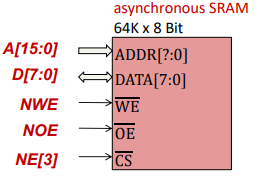
\includegraphics[width=\linewidth]{sram_pins_ex.png}
    \end{minipage}
    


    \paragraph{Basisadresse + Anzahl Adressen}
    \begin{itemize}
        \item Basisadresse: niedrigste Adresse des Bausteins
        \item Höchste Adresse: Basisadresse + Speichergröße - 1
        \item Beispiel 64K: 64K = 64 $\times$ 1024 = 65536 = 0x10000
    \end{itemize}
    
    \paragraph{Partial Address Decoding}
    \begin{itemize}
        \item Nicht alle Adressleitungen werden dekodiert
        \item Führt zu mehreren gültigen Adressbereichen (Aliasing)
        \item Anzahl Bereiche = $2^{nicht\_dekodierte\_Bits}$
    \end{itemize}
    
    
\end{concept}

\begin{example2}{Connecting Asynchronous SRAM to STM32F4}\\
A 64K × 8-bit asynchronous SRAM chip needs to be connected to the FMC of an STM32F429 microcontroller. The address 0x6800'0000 should be the lowest address used to access the memory.

Answer:
\begin{enumerate}
    \item How many address pins does the memory need?
    \item Which FMC signals should be connected to the SRAM chip?
    \item At what address is the highest byte of the memory accessed?
    \item Explain why the same memory location can be accessed at multiple addresses.
\end{enumerate}

\tcblower

1. \textbf{Number of address pins:}
   \begin{itemize}
     \item Memory size = 64K = 2$^{16}$ bytes
     \item Need 16 address lines: ADDR[15:0]
   \end{itemize}

2. \textbf{FMC signals to connect:}
   \begin{itemize}
     \item Address lines: A[15:0]
     \item Data lines: D[7:0] (8-bit data bus)
     \item Chip select: NE[3] (for Bank 3 based on address 0x6800'0000)
     \item Output Enable: NOE
     \item Write Enable: NWE
   \end{itemize}

3. \textbf{Highest memory address:}
   \begin{itemize}
     \item Lowest address: 0x6800'0000
     \item Memory size: 64K = 0x10000 bytes
     \item Highest address: 0x6800'0000 + 0xFFFF = 0x6800'FFFF
   \end{itemize}

4. \textbf{Multiple address access:}
   \begin{itemize}
     \item This occurs due to partial address decoding
     \item Only address lines A[15:0] are connected to the memory chip
     \item Higher address bits A[25:16] are not decoded/connected
     \item Any address where A[27:26] = 01 (Bank 2) and A[15:0] match will access the same memory location
     \item \textbf{Aliasing-Bereiche:} 0x68XX'0000, 0x69XX'0000, 0x6AXX'0000, 0x6BXX'0000
     \item The number of 64KB address blocks that map to the same memory is 2$^{10}$ = 1024 (from the 10 undecoded bits A[25:16])
   \end{itemize}
\end{example2}

\begin{example2}{Address Space Calculation for External Memory}\\
Calculate the address range for an external 32K x 8-bit SRAM connected to FMC bank 3.
\tcblower
For an external SRAM connected to FMC bank 3:
\vspace{1mm}\\
1. Base address of FMC bank 3 = 0x68000000\\
2. Memory size = 32K bytes = 32,768 bytes = 0x8000 bytes
\vspace{3mm}\\
Therefore, the address range for this SRAM would be:\\
- Start address: 0x68000000\\
- End address: 0x68000000 + 0x8000 - 1 = 0x68007FFF
\vspace{3mm}\\
Address range: 0x68000000 - 0x68007FFF
\vspace{3mm}\\
Note: Due to partial address decoding, this SRAM might also be accessible at other addresses within bank 3. For example, it might also respond to addresses:\\
0x68008000 - 0x6800FFFF, 0x68010000 - 0x68017FFF, etc.
\end{example2}

\begin{example2}{Memory Access and Address Decomposition} 
    A 16-bit wide asynchronous SRAM is connected to the FMC of an STM32F429 microcontroller. Analyze what happens when the CPU writes a single byte to address 0x6402'8F21:
    \paragraph{Determine Memory Device}
    \begin{itemize}
     \item Address 0x6402'8F21 begins with 0x64...
     \item From address bits [27:26] = 01, this is in Bank 2
     \item This activates NE2 (chip select 2)
   \end{itemize}
    \textbf{External SRAM, Device 2 (NE2)}:\\
    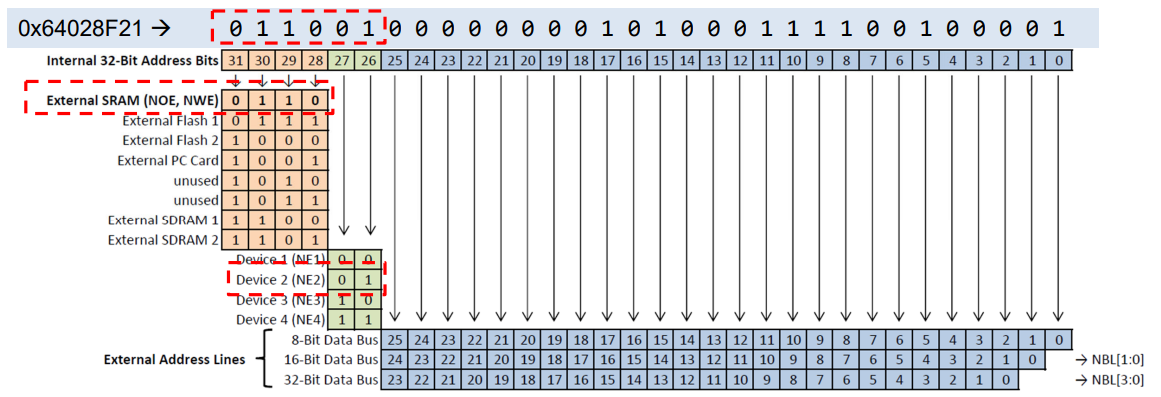
\includegraphics[width=\linewidth]{addrecskfdjdklfhkldshsd.png}

    \paragraph{Determine Memory Location}
       \begin{itemize}
     \item Only address bits [25:1] are passed to the SRAM device
     \item Bit [0] is used to select the high/low byte within a 16-bit word
     \item \textbf{Memory location = 0x0014'7490} (shifted right by 1 bit and ignoring higher bits that aren't connected)
   \end{itemize}
    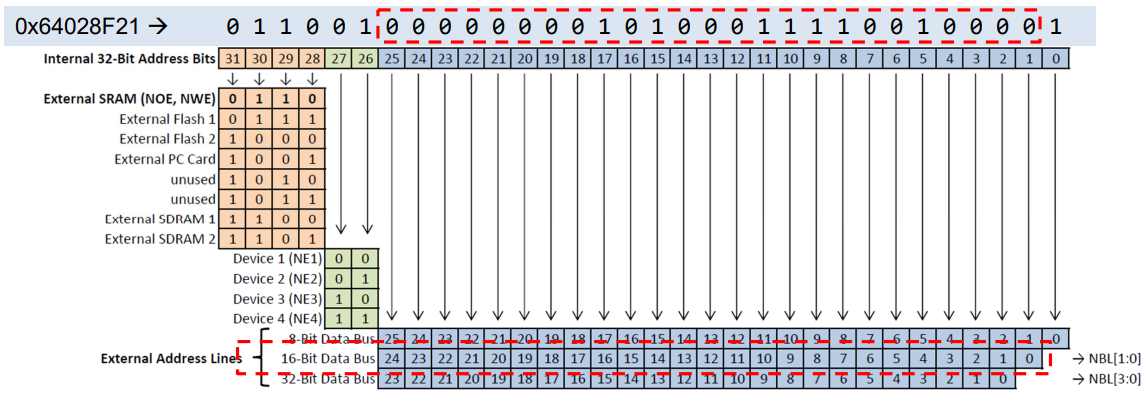
\includegraphics[width=\linewidth]{decompex3.png}

    \paragraph{Determine Byte Line}
       \begin{itemize}
     \item Address bit [0] = 1, so we're accessing the high byte in the 16-bit word
     \item For 16-bit memory: NBL[1:0] = 10 (high byte active)
     \item NBL[0] = 1 (not active), NBL[1] = 0 (active) $\rightarrow$ select high byte
   \end{itemize}
    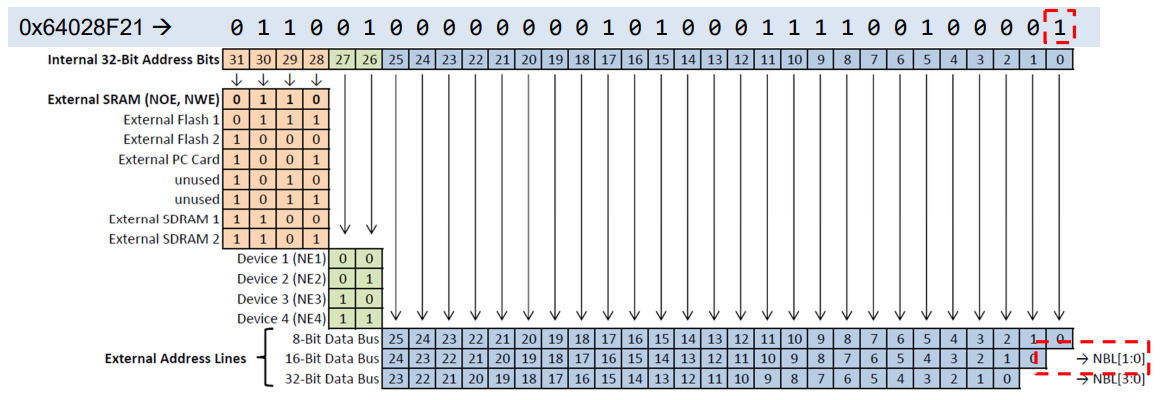
\includegraphics[width=\linewidth]{addressdecompbyteline.png}
\end{example2}

\begin{example2}{Memory Access and Address Decomposition continued}
    \paragraph{Address Decomposition}
    Address 0x64028F21:
    \begin{itemize}
        \item Determine Memory Device $\rightarrow$ External SRAM, Device 2 (NE2)
        \item Determine Memory Location $\rightarrow 0 \times 0014790$
        \item Determine Byte Line $\rightarrow$ NBL[0] = 1, NBL[1] =0, i.e., select high byte
    \end{itemize}
    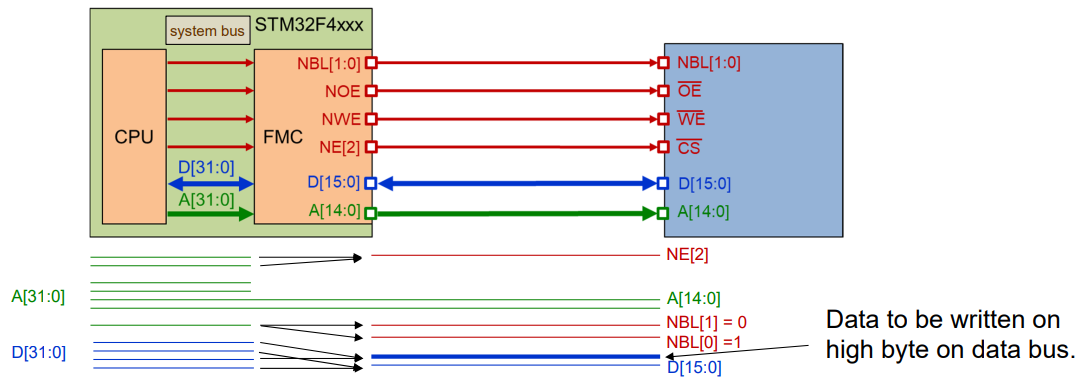
\includegraphics[width=\linewidth]{addressdecompex.png}
       \begin{itemize}
     \item 0x6402'8F21 decomposed:
     \begin{itemize}
       \item Bits [31:28]: 0x6 (not used for decoding)
       \item Bits [27:26]: 01 (Bank 2, activates NE2)
       \item Bits [25:1]: Memory address within SRAM (0x0014'7490)
       \item Bit [0]: 1 (select high byte)
     \end{itemize}
     \item FMC signals during access:
     \begin{itemize}
       \item NE2 = 0 (active)
       \item A[24:0] = 0x0014'7490 (memory address)
       \item NBL[1:0] = 10 (access high byte)
       \item NWE = 0 (active, writing)
       \item Data appears on D[15:8] (high byte)
     \end{itemize}
   \end{itemize}
\end{example2}



